\chapter[Inteligencia del Cliente]{Inteligencia del Cliente}
\label{ch:ic}

\section{Inteligencia del Cliente}
\subsection{¿Qué es Inteligencia del Cliente?}

El proceso de Inteligencia del Cliente (Customer Intelligence, CI), gestiona, almacena y analiza datos e información relacionada a los clientes, buscando un mayor entendimiento de sus necesidades, para así mejorar el flujo de comunicación, el servicio prestado y diseñar y/o preparar decisiones estratégicas concretas.\cite{ic}\\

En otras palabras, consiste en convertir los datos en bruto con los que se cuentan, en información científica útil y analizable. \cite{ic}\\

Una gestión adecuada de CI, trae consigo beneficios para la empresa u organización. Mejorando la experiencia del servicio al cliente, toma estratégica de decisiones y predicción de hábitos o comportamiento del cliente.\cite{ic}\\

Inteligencia del Cliente está fuertemente relacionado a la ``Gestión de Relación con el Cliente'' (Customer Relationship Management, CRM), CI es un componente clave para CRM, ya que CI capta datos e información del cliente que CRM no logra hacer. CI se basa en apreciaciones, opiniones del cliente, principalmente en aspectos de emociones que provoca el servicio y/o producto entregado por la empresa. En cambio, un sistema tradicional de CRM obtiene los datos e información del cliente basado en historiales, como por ejemplo historial de compras. Aplicando ambos conceptos de manera efectiva, CI otorga una importante fuente de información con respecto a comportamiento y experiencia de los clientes de una empresa.\cite{wikiic}\\



\subsection{Estructura de Relacionamiento y CRM}

Inteligencia del Cliente estudia, desde los ámbitos psicológicos y sociales al ser humano y su forma de relacionarse con el resto, ya que busca como objetivo relacionar los clientes con la empresa, tal como relacionarse con otro ser humano, generando un compromiso con una carga emocional.\\


La gestión de relación con el cliente CRM, es parte de una estrategia centrada en el cliente, una parte fundamental de su idea, es la recopilación de la mayor cantidad de información posible de los clientes, para poder entender sus necesidades y dar valor a la oferta.\cite{crm}\\


Los sistemas informáticos ayudan a gestionar la relación con el cliente, almacenando sus datos y aplicando Inteligencia de Negocio en conjunto con minería de datos.

\subsection{Metodología de la Metáfora}

La metodología de la metáfora es una herramienta del marketing que analiza el pensamiento consciente e inconsciente del consumidor, teniendo en cuenta puntos de neurociencia y psicología con el objetivo de comprender sus emociones y motivaciones, ya que están estrechamente relacionadas con los procesos del razonamiento y por ende las emociones contribuyen a una toma de decisiones sólidas.\footnote{``Viaje desde lo conocido'', Zalman Cap. 1}\\

En marketing, se piensa que el consumidor capta sus recuerdos como una cámara, un mecanismo que capta imágenes, pero con un toque de creatividad, lo que hace el recuerdo maleable, es decir, cambian constantemente de forma inconsciente, haciendo que los recuerdos sean metáforas. \\

Cuando los consumidores usan las metáforas para describir un producto o servicio llevan sus pensamientos y sentimientos inconsciente a un nivel de consciencia que permite encontrar sentido a lo que descubren e influye en sus decisiones y acciones. Esto permite a las empresas y organizaciones diseñar ofertas más valiosas para los consumidores.\footnote{``Interrogar a la mente'', Zalman Cap. 4}\\

En las ciencias cognitivas el captar o inferir el pensamiento de una persona a través de sus declaraciones o conductas es conocido como ``constructos''. Los constructos no son el pensamiento ni la conducta real de la persona, más bien es una interpretación que realiza en este caso el mercadólogo del consumidor.\footnote{``Pensándolo bien'', Zalman Cap. 6}\\

Los constructos son más bien etiquetas que realiza una persona, a partir del análisis del comportamiento de otra. Los constructos pueden tener asociaciones entre si, generando un ``mapa de consenso''. Un mapa de consenso nace a partir de los constructos de un grupo de personas, y se trata de un gráfico de pensamientos y sentimientos compartidos de un grupo sobre un tema en concreto. Figura \ref{fig:consenso}


\begin{figure}[h]
\begin{minipage}{\textwidth} 
\centering 
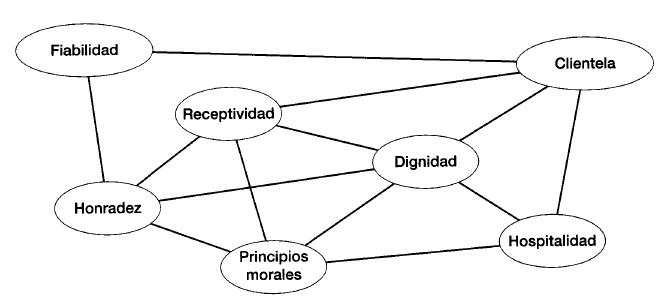
\includegraphics[width=10cm,height=5cm] {consenso.png} 
\caption[Mapa de Consenso]{Mapa de Consenso~\footnote{Fuente: Mind of the Market Laboratory/Harvard Business School}}
\label{fig:consenso}
\end{minipage}
\end{figure}

La metodología de la metáfora se aplica en entrevistas, las cuales pueden ir variando dependiendo del objetivo de la investigación, para el trabajo que se realizará en esta investigación, se seguirán los siguientes pasos:\\

\begin{enumerate}
\item Recolección de revistas o periódicos con muchas imágenes.
\item Pedir al entrevistado que recorte imágenes que se relacionen o motiven sobre un tema en concreto.
\item Pedir que describan las imágenes recortadas y luego las agrupen en distintos grupos, señalando un tema por grupo.
\item Realizar una pregunta opuesta al tema en concreto y tomar apuntes respecto a las respuestas.
\item Definir constructos a partir de las apreciaciones que se obtuvieron con las descripciones de las imágenes y respuestas de la pregunta opuesta.
\item Identificar relaciones entre los constructos definidos y crear un mapa de consenso.
\item Generar métricas y variables a partir de los constructos y sus asociaciones.

\end{enumerate}

\section{Inteligencia de Negocio}

Inteligencia de Negocio (Business intelligence, BI), es el proceso que permite transformar los datos en información y la información en conocimiento, permitiendo ayudar a la empresa u organización en la toma de decisiones.\cite{bi}\\

BI nace debido a la gran cantidad de datos que manejan las organizaciones, lo que, a través de la combinación de tecnología, herramientas y procesos, logra la transformación de datos. Dentro de las tecnologías utilizadas en las empresas, se pueden identificar dos tipos de sistemas, los sistemas OLTP que proporcionan datos de orígenes y los sistemas OLAP que ayudan a analizar dichos datos: \cite{olapvsoltp}\\


\begin{enumerate}

    \item \textbf{Sistemas OLTP (Online Transaccional Processing, Procesamiento Transaccional en Línea):}\\
Son bases de datos orientadas al procesamiento de transacciones cortas, rápidas y en línea. Una transacción genera un proceso atómico (que debe ser validado con un commit, o invalidado con un rollback), y que puede involucrar operaciones de inserción (INSERT), modificación (UPDATE) y borrado (DELETE) de datos.\\

\item \textbf{Sistemas OLAP (Online Analytical Processing, Procesamiento Analítico en Línea):}\\
Un sistema OLAP es un vector multidimensional, de N dimensiones, en el, la información se almacena en cada una de estas dimensiones, de forma ordenada y jerarquizada, lo cual ayuda a realizar un análisis rápido de su contenido. Las dimensiones de OLAP son diferentes perspectivas de análisis de información, en donde el usuario especifica diversos criterios que definen cuál y de qué forma será presentada, acumulada y ordenada la información, obteniendo resultados a una velocidad superior e la que se obtendría con un sistema de bases de datos relacional.\\

Las acciones básicas que tienen las tecnologías que implementan un sistema OLAP son: \cite{bi}

\begin{itemize}
    \item Segmentar: Agrupar datos por condiciones especificadas.\\
\item Filtrar: genera informes de datos acotados por algún parámetro.\\
\item Profundizar (Drill down): Desglose de un dato, ejemplo, el desglose de un semestre, sería el mes.\\
\item Sintetizar (Drill up): Deshace el desglose de ``Profundizar''.\\
\item Rotar (Drill anywhere): Realiza un desglose por una característica de una jerarquía distinta a la que se está visualizando actualmente.\\

    
\end{itemize}
    
\end{enumerate}

    Cada uno de estos sistemas están hechos para realizar una tarea específica, por lo cual, a pesar de que ambas son bases de datos, tienen diferencias. A continuación se detallan las principales diferencias entre los sistemas OLTP y OLAP, Tabla \ref{tabla:oltpvsolap}.

\begin{table}[H]
\centering
\begin{tabular}{|c|c|}
\hline
OLTP & OLAP\\ \hline
Son la fuente original de los datos & Los datos OLAP provienen de OLTP \\ \hline
Actualización en tiempo real &	Solo realiza procesos de carga \\ \hline
Por lo general muy rápidos & Lento debido a la gran cantidad de datos a procesar \\ \hline
Consultas simples y estandarizadas & Consultas complejas \\ \hline
Bases de datos normalizadas &	Bases de datos desnormalizadas \\ \hline
Utilizan poco espacio & Requiere una gran cantidad de espacio \\ \hline
\end{tabular}\newline
\caption{Diferencias OLTP vs OLAP. \cite{tablaolapvsoltp}}
\label{tabla:oltpvsolap}
\end{table}

Los sistemas OLTP se pueden utilizar de manera independiente de OLAP, sin embargo, cuando una empresa maneja grandes cantidades de datos, es necesario utilizar una arquitectura que involucra ambos sistemas. Arquitectura que maneja los siguientes componentes:


\begin{itemize}
    \item Bases Operacionales (OLTP).
    \item Procesos ETL
    \item Área Staging
    \item Base Analítica (Data Warehouse)
    \item Herramientas de gestión
\end{itemize}

Estos componentes son los que conforman el proceso de Inteligencia de Negocio, y se puede visualizar en el siguiente esquema, Figura \ref{fig:esquemaBI} :

\begin{figure}[H]
\begin{minipage}{\textwidth}
\centering 
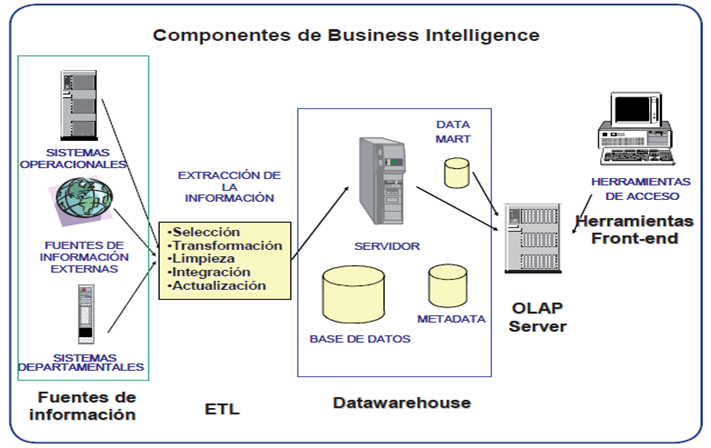
\includegraphics[width=12cm,height=7cm] {componentesBI.png}
\caption[Esquema de Inteligencia de Negocio]{Esquema de Inteligencia de Negocio~\footnote{Curso Inteligencia de Negocios 2/2015, UDP}}
\label{fig:esquemaBI}
\end{minipage}
\end{figure}

\subsection{Bases Operacionales}

Las bases operacionales son las encargadas de almacenar todos los datos de transacciones de una organización, datos que pueden ser de diferentes fuentes, por ejemplo, bases de datos Oracle, SQL Server, Excel entre otros.

\subsection{Procesos ETL}

Los procesos ETL (del inglés, Extract, Transform, Load) son una pieza fundamental de la Inteligencia de Negocio, ya que trata del proceso de mover datos de múltiples fuentes, transformar y luego cargar en otra base de datos.\\

Estos procesos consumen entre el 60 \% y 80 \% del tiempo de un proyecto de BI, y son proceso clave en la vida del proyecto.\cite{etl}\\

ETL se divide en 5 subprocesos:

\begin{enumerate}
\item Extracción:
Recupera los datos necesarios físicamente de las distintas fuentes de información, dejando los datos en bruto. Su extracción puede ser manual o utilizando una herramienta. Sus principales problemas son las distintas fuentes de datos y distintas plataformas.

\item Limpieza:
Recupera los datos en bruto y comprueba su calidad, elimina los duplicados y, cuando es posible, corrige los valores erróneos, si existen valores vacíos, los completa siempre y cuando sea posible.\\

Estos valores, generalmente se llaman valores sucios, y es muy probable encontrarlos, lo importante es saber el origen de dicha suciedad.\\

La limpieza se divide en distintas etapas:
\begin{itemize}
    \item Depurar los valores:
    Localiza elementos individuales de las fuentes de datos y los aísla en estructura de destino, por ejemplo, Dirección $\rightarrow $ calle, número, comuna, ciudad.
    
    \item Corregir:
    Corrige los datos individuales utilizando algoritmos y fuentes de datos externas.
    
    \item Estandarizar:
    Se trabaja con formatos de datos definidos y se aplican rutinas para homogeneizar datos. 
    
    \item Relacionar:
    Busca y relaciona los valores de los registros, corrigiéndolos y estandarizándolos según reglas del negocio, eliminando datos duplicados.
    
    \item Consolidar: 
    Analiza e identifica relaciones entre registros relacionados y los junta en una sola representación.

\end{itemize}

\item Transformación:
Recupera los datos limpios y de alta calidad, los estructura y suma en distintos modelos de análisis.

\item Integración:
Valida que los datos cargados son consistentes con las definiciones y formatos de la base analítica. Integra los datos en los distintos modelos de las distintas áreas de negocio que se han definido.

\item Actualización:
Se añaden los datos a la base analítica.


\end{enumerate}


\subsection{Área Staging}

El área staging es una base de datos la cual es una copia de todas las bases operacionales, generada principalmente para realizar las siguientes actividades:

\begin{itemize}
    \item Facilitar extracción de datos.
    \item Limpiar y mejorar la calidad de los datos.
    \item Operar y ejecutar procesos sin afectar el funcionamiento de las bases operacionales.
\end{itemize}

\subsection{Base Analítica (Data Warehouse)}

La base analítica o Data Warehouse es un repositorio o colección de datos orientada a un tema, integrada, variante en el tiempo y no volátil, que apoya el proceso de toma de decisiones de gestión.\\

En la base analítica se almacenan todos los datos procesados de Área Staging y ETL.\\

Un Data Warehouse puede tener varios DataMart, un DataMart son pequeños Data Warehouse que almacenan datos específicos de un área de negocio o departamento de una empresa.\\

A continuación se detallan las principales diferencias entre las bases operacionales y las bases analíticas, Tabla \ref{tabla:bdovsbda}. 

\begin{table}[H]
	\begin{minipage}{\textwidth} 
		\centering
		\begin{tabular}{ | c | c |}
			\hline
			BD Operacional & BD Analítica\\ \hline
			De transacciones & De consultas masivas \\ \hline
			Predomina la actualización & Predomina la consulta \\ \hline
			Actualizable & Carga, pero no actualiza \\ \hline
			De tipo operativo & Análisis y toma de decisiones \\ \hline
			Datos normalizados & Datos en estrella o copo de nieve \\ \hline
			Usuarios de perfiles medios o bajos & Usuarios de perfiles altos \\ \hline
			Estructura normalmente relacional & Visión multidimensional\\ \hline
		\end{tabular}\newline
		\caption[Diferencias BD Operacional vs BD Analítica.]{Diferencias BD Operacional vs BD Analítica.~\footnote{Creación propia}}
		\label{tabla:bdovsbda}
	\end{minipage}
\end{table}


Las bases analíticas están diseñados y desarrollados para realizar consultas complejas dentro de un volumen muy grande de datos, para lo cual se necesita una arquitectura para cumplir con este propósito, existen 3 arquitecturas, MOLAP (Multidimensional), ROLAP (Relacional) y HOLAP (Híbrido), la más usada es el modelo multidimensional.\\

Los modelos multidimensionales tienen 3 conceptos principales:

\begin{itemize}
    \item Unidad de Medida:
    Atributo cuantificable asociado a los hechos. Ejemplos, Volumen de las ventas, número de transacciones efectuadas, porcentaje de beneficios.
    
    \item Tabla de Hecho:
    Tabla que almacena los valores detallados para medidas, permite realizar inserciones entre las dimensiones y las medidas.
    
    \item Dimensiones:
    Son tablas que permiten la agrupación de los hechos.

\end{itemize}

Las bases multidimensionales son utilizadas con dos esquemas:

\begin{enumerate}
	\item Esquema Estrella:
	Es un esquema simple que utiliza una tabla de hecho, una o más tablas de dimensiones desnormalizadas, que están unidas con la tabla de hecho, Figura \ref{fig:estrella}.
	
	\begin{figure}[H]
		\begin{minipage}{\textwidth} 
			\centering 
			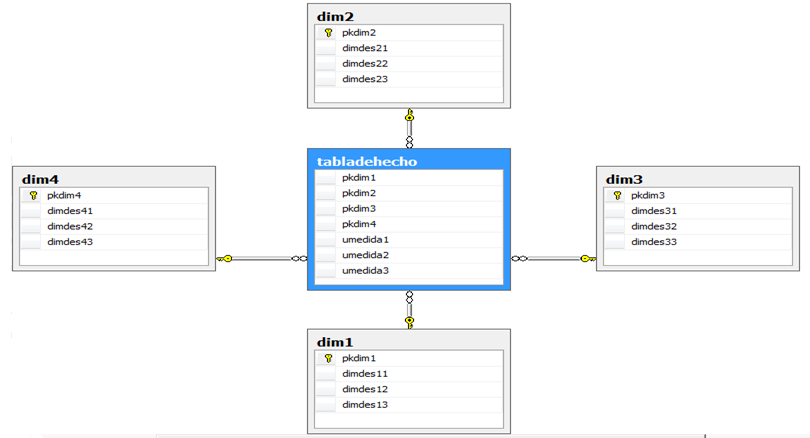
\includegraphics[width=12cm,height=7cm] {estrella.png} 
			\caption[Esquema Estrella]{Esquema Estrella~\footnote{Curso Inteligencia de Negocios 2/2015, UDP}}
			\label{fig:estrella}
		\end{minipage}
	\end{figure}
	
	\item Esquema Copo de Nieve:
	Es un esquema complejo, derivado del esquema estrella, las tablas de dimensiones se encuentran normalizadas en múltiples tablas, y la tabla de hecho no es la única que establece uniones con las otras tablas, Figura \ref{fig:copo}.
	
	\begin{figure}[h]
		\begin{minipage}{\textwidth} 
			\centering 
			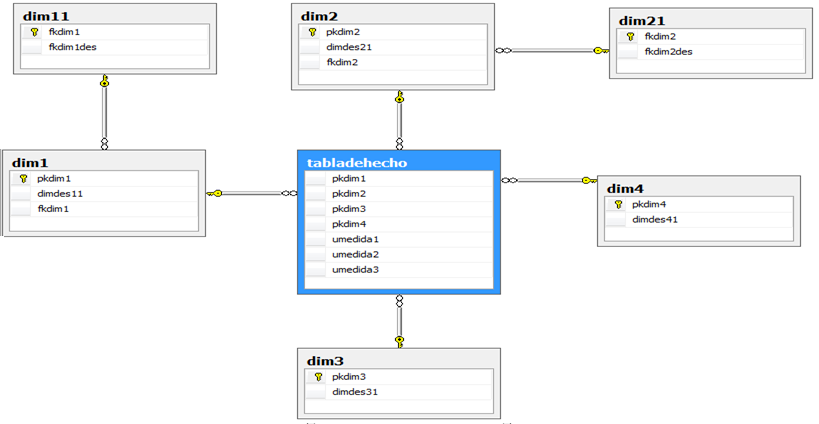
\includegraphics[width=12cm,height=7cm] {copo.png} 
			\caption[Esquema Copo de Nieve]{Esquema Copo de Nieve~\footnote{Curso Inteligencia de Negocios 2/2015, UDP}}
			\label{fig:copo}
		\end{minipage}
	\end{figure}
	
\end{enumerate}


\subsection{Herramientas de Gestión}

Después de que los datos son procesados y almacenados en la base analítica, estos se encuentran disponibles para ser visualizados y analizados a través de herramientas de gestión, que permiten a las personas de alto mando dentro de una organización tener la información de forma rápida y oportuna para la toma de decisiones. Existen una variedad de herramientas que cumplen diferentes objetivos, a continuación se identifican alguna de ellas.

\subsubsection{Query $\&$ Reporting}

Son herramientas que realizan consultas o informes que trabajan tanto sobre el detalle como sobre las agregaciones de la información. Manejan una gran cantidad de información y principalmente responden a la pregunta ¿Qué sucedió?

\subsubsection{Análisis OLAP}

Las herramientas de análisis OLAP o ``Analytics Reports'' son utilizadas por los analistas que necesitan tener la información desde distintos puntos de vistas. Estas herramientas permiten navegar dentro de la información profundizando o ir al detalle, conocidos como navegación jerárquica (Drill Down) y navegación al detalle (Drill Through). Estas herramientas responden a la pregunta ¿Por qué sucedió?

\subsubsection{Dashboard}

Las herramientas de dashboard totaliza los datos, los cuales generalmente están representados en gráficas que representan el estado actual del negocio. La totalización de datos se representa como KPIs (Key Performance Indicator), en español, indicadores claves de desempeño, que son valores relacionados con un objetivo fijado de antemano por la organización y normalmente se expresa en porcentaje, sirven para visualizar el progreso en un aspecto concreto. Por ejemplo, una representación gráfica comúnmente usada es el semáforo, el cual puede representar las ventas del mes de una empresa fijando indicadores acordes a los objetivos de ventas, si el objetivo es alcanzar las 100 ventas en un mes, si se está cumpliendo con dicho objetivo o más el semáforo estará en color verde, si es menor a 100 estará en amarillo y si es menor a una cantidad definida ejemplo 70, entonces se encontrará en color rojo.\\

Estas herramientas son las más usadas por los ejecutivos o personal de alto rango dentro de una organización, ya que permite monitorear tiempo real la situación actual de la organización, facilitando la toma de decisiones. Estas herramientas responden a la pregunta ¿Qué está sucediendo?


\subsubsection{Data Mining o Minería de Datos}

Las herramientas de data mining realizan análisis de datos históricos de la organización, con el objetivo de buscar patrones que predigan el comportamiento o acción de un suceso o persona. Para esto realiza acciones de clasificación, segmentación o predicción. Por ejemplo, el análisis de las ventas de los últimos 5 años permite estimar una aproximación de las ventas del año actual. Estas herramientas responden a la pregunta ¿Qué va a suceder?




